\documentclass{standalone}

\usepackage{tikz}

\usepackage{unicode-math}
\newcommand\dd{\mathrm{d}}

\begin{document}
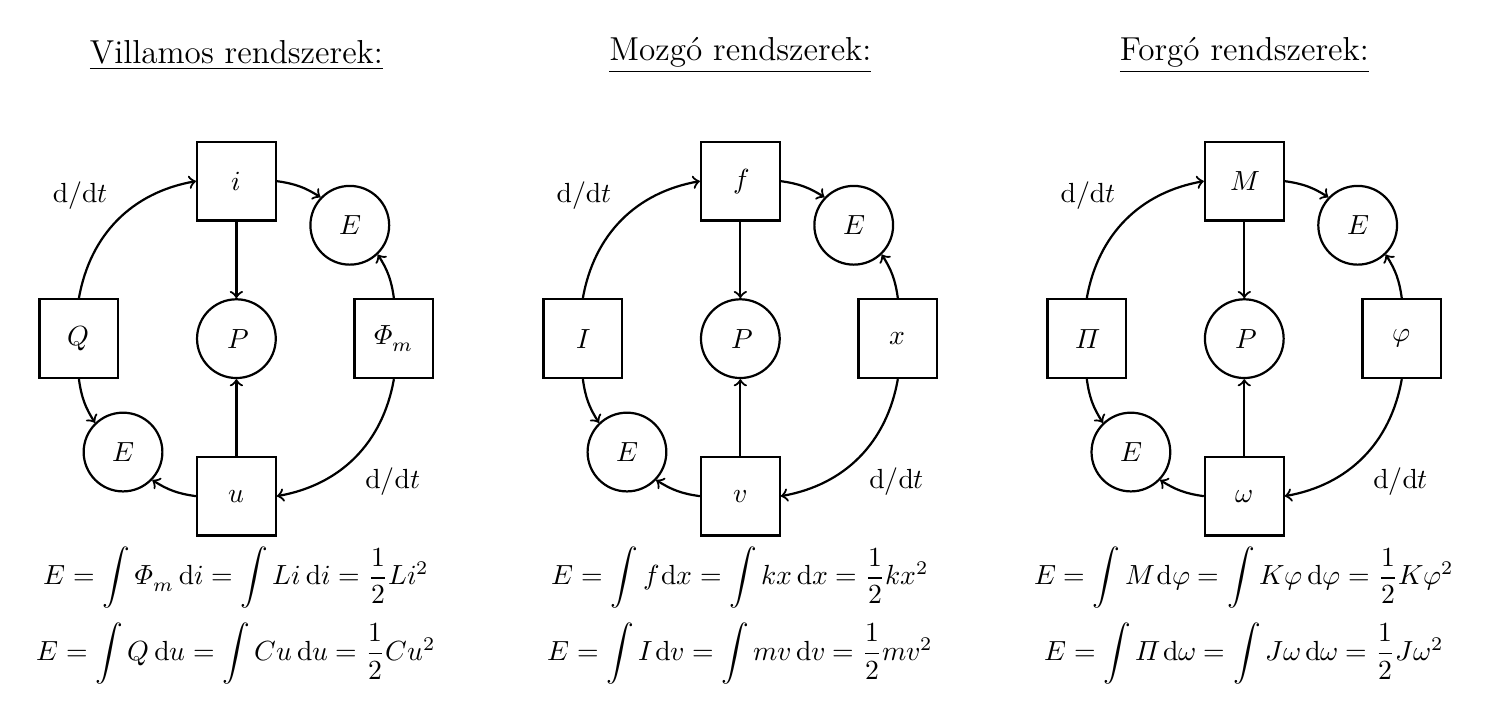
\begin{tikzpicture}[
    thick, scale=.8,
    rect/.style={rectangle, draw=black,minimum width=1cm, minimum height=1cm},
    circ/.style={circle, draw=black,minimum width=1cm, minimum height=1cm},
  ]
  \foreach \x/\u/\l/\r/\d/\n/\teq/\beq in {
  0cm/i/Q/\varPhi_m/u/Villamos/{
  \int \varPhi_m \, \dd i = \int L i \, \dd i = \frac{1}{2}Li^2
  }/{
  \int Q \, \dd u = \int C u \, \dd u = \frac{1}{2}Cu^2
  },
  8cm/f/I/x/v/Mozgó/{
  \int f \, \dd x = \int kx \, \dd x = \frac{1}{2}kx^2
  }/{
  \int I \, \dd v = \int mv \, \dd v = \frac{1}{2}mv^2
  },
  16cm/M/\itPi/\varphi/\omega/Forgó/{
  \int M \, \dd \varphi = \int K \varphi \, \dd \varphi = \frac{1}{2}K\varphi^2
  }/{
  \int \itPi \, \dd \omega = \int J \omega \, \dd \omega = \frac{1}{2}J\omega^2
  }
  }{
  \begin{scope}[xshift=\x]
    \node[rect] (u) at (0,2.5) {$\u$};
    \node[rect] (l) at (-2.5,0) {$\l$};
    \node[rect] (r) at (2.5,0) {$\r$};
    \node[rect] (d) at (0,-2.5) {$\d$};
    \node[circ] (m)  at (0,0) {$P$};
    \node[circ] (e1) at (-1.8,-1.8) {$E$};
    \node[circ] (e2)at (+1.8,+1.8) {$E$};

    \draw[-to] (u) -- (m);
    \draw[-to] (d) -- (m);
    \draw[-to] (l.north) to[bend left=35] node[midway, above left] {$\mathrm{d/d}t$} (u.west);
    \draw[-to] (r.south) to[bend left=35] node[midway, below right] {$\mathrm{d/d}t$} (d.east);
    \draw[-to] (d.west) to[bend left=12.5] (e1);
    \draw[-to] (l.south) to[bend right=12.5] (e1);
    \draw[-to] (u.east) to[bend left=12.5] (e2);
    \draw[-to] (r.north) to[bend right=12.5] (e2);

    \node[] at (0,-3.8) {$E = \displaystyle\teq$};
    \node[] at (0,-5.0) {$E = \displaystyle\beq$};A
    \node at (0,4.5) {\large \underline{\n{} rendszerek:}};
  \end{scope}
  }
\end{tikzpicture}
\end{document}
